\documentclass{article}

\usepackage{fancyhdr}
\usepackage{extramarks}
\usepackage{amsmath}
\usepackage{amsthm}
\usepackage{amsfonts}
\usepackage{tikz}
\usepackage{physics}
\usepackage{amssymb}
\usepackage[plain]{algorithm}
\usepackage{algpseudocode}

\usetikzlibrary{automata,positioning}

%
% Basic Document Settings
%

\topmargin=-0.45in
\evensidemargin=0in
\oddsidemargin=0in
\textwidth=6.5in
\textheight=9.0in
\headsep=0.25in

\linespread{1.1}

\pagestyle{fancy}
\lhead{\hmwkAuthorName}
\chead{\hmwkClass\ : \hmwkTitle}
\rhead{\firstxmark}
\lfoot{\lastxmark}
\cfoot{\thepage}

\renewcommand\headrulewidth{0.4pt}
\renewcommand\footrulewidth{0.4pt}

\setlength\parindent{0pt}

%
% Create Problem Sections
%

\newcommand{\enterProblemHeader}[1]{
    \nobreak\extramarks{}{Problem \arabic{#1} continued on next page\ldots}\nobreak{}
    \nobreak\extramarks{Problem \arabic{#1} (continued)}{Problem \arabic{#1} continued on next page\ldots}\nobreak{}
}

\newcommand{\exitProblemHeader}[1]{
    \nobreak\extramarks{Problem \arabic{#1} (continued)}{Problem \arabic{#1} continued on next page\ldots}\nobreak{}
    \stepcounter{#1}
    \nobreak\extramarks{Problem \arabic{#1}}{}\nobreak{}
}

\setcounter{secnumdepth}{0}
\newcounter{partCounter}
\newcounter{homeworkProblemCounter}
\setcounter{homeworkProblemCounter}{1}
\nobreak\extramarks{Problem \arabic{homeworkProblemCounter}}{}\nobreak{}

%
% Homework Problem Environment
%
% This environment takes an optional argument. When given, it will adjust the
% problem counter. This is useful for when the problems given for your
% assignment aren't sequential. See the last 3 problems of this template for an
% example.
%
\newenvironment{homeworkProblem}[1][-1]{
    \ifnum#1>0
        \setcounter{homeworkProblemCounter}{#1}
    \fi
    \section{Problem \arabic{homeworkProblemCounter}}
    \setcounter{partCounter}{1}
    \enterProblemHeader{homeworkProblemCounter}
}{
    \exitProblemHeader{homeworkProblemCounter}
}

%
% Homework Details
%   - Title
%   - Due date
%   - Class
%   - Section/Time
%   - Instructor
%   - Author
%

\newcommand{\hmwkTitle}{Assignment\ \#1}
\newcommand{\hmwkDueDate}{Due 31st August 2018}
\newcommand{\hmwkClass}{Classical Mechanics}
\newcommand{\hmwkClassTime}{}
\newcommand{\hmwkClassInstructor}{Prof.Manas Kulkarni}
\newcommand{\hmwkAuthorName}{\textbf{Aditya Vijaykumar}}

%
% Title Page
%

\title{
    %\vspace{2in}
    \textmd{\textbf{\hmwkClass:\ \hmwkTitle}}\\
    \normalsize\vspace{0.1in}\small{\hmwkDueDate\ }\\
%    \vspace{3in}
}

\author{\hmwkAuthorName}
\date{}

\renewcommand{\part}[1]{\textbf{\large Part \Alph{partCounter}}\stepcounter{partCounter}\\}

%
% Various Helper Commands
%

% Useful for algorithms
\newcommand{\alg}[1]{\textsc{\bfseries \footnotesize #1}}

% For derivatives
\newcommand{\deriv}[1]{\frac{\mathrm{d}}{\mathrm{d}x} (#1)}

% For partial derivatives
\newcommand{\pderiv}[2]{\frac{\partial}{\partial #1} (#2)}

% Integral dx
\newcommand{\dx}{\mathrm{d}x}

% Alias for the Solution section header
\newcommand{\solution}{\textbf{\large Solution}}

% Probability commands: Expectation, Variance, Covariance, Bias
\newcommand{\E}{\mathrm{E}}
\newcommand{\Var}{\mathrm{Var}}
\newcommand{\Cov}{\mathrm{Cov}}
\newcommand{\Bias}{\mathrm{Bias}}

\begin{document}

\maketitle

%\pagebreak

\begin{homeworkProblem}
\textbf{Part (a)}
\begin{flalign*}
V(x) = \alpha x^2/2 + \beta x^4/4\\
F(x) = -\pdv{V}{x} = -\alpha x - \beta x^3
\end{flalign*}
Including the damping term, we write the equation of motion as,
$$m\ddot{x} + \delta \dot{x} = -\alpha x - \beta x^3$$
$$m\ddot{x} + \delta \dot{x} + \alpha x + \beta x^3 = 0$$

The total energy of the system $E=T+V=m\dot{x}^2/2 + \alpha x^2/2 + \beta x^4/4$. Taking the time derivative, one gets
$$\dot{E} = m\ddot{x}\dot{x} + \alpha x \dot{x} + \beta x^3\dot{x}$$
Substituting from the equation of motion for $m\ddot{x}$,
$$\dot{E}=-(\delta \dot{x} + \alpha x + \beta x^3)\dot{x} + \alpha x \dot{x} + \beta x^3\dot{x}$$
$$\dot{E} = -\delta \dot{x}^2$$
Hence energy is dissipated from the system at a rate $\delta \dot{x}^2$.\\

\textbf{Part (b)}\\
The potential is plotted in in Figure 1. We see that for $\alpha = - 0.25$ and $\beta = -0.25$, there is only one critical point (maxima). So whatever energy is provided, the particle will not settle to a stable equilibrium point.

\begin{figure}[!h]
	\label{1a}
	\caption{Plots of $V(x)$ for different parameters}
	\centering
	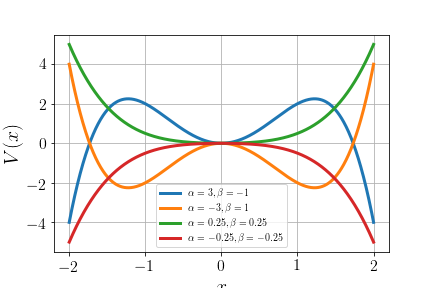
\includegraphics[scale=0.7]{1.png}
\end{figure}

Now for the qualitative description of motion in various cases,
\begin{itemize}
	\item $\alpha > 0$ and $\beta > 0$ - There is just one equilibrium point at $x=0$, and it is a stable equilibrium point. A particle in this potential with a finite kinetic energy will exhibit periodic motion.
	
	\item  $\alpha > 0$ and $\beta > 0$ - There is just one equilibrium point at $x=0$, and it is an unstable equilibrium point. A particle at the origin will run off to infinity even if disturbed slightly. If the particle starts anywhere else, it will cross the potential barrier (ie. $x=0$) or not depending on whether it has enough energy.  Nevertheless, the particle will fly off to one of the infinities.This won't happen only if it is given exactly the amount of energy such that it stays at rest at $x=0$.
	
	\item  $\alpha > 0$ and $\beta < 0$ - There are two unstable and one stable equilibrium point ($x=0$). If the initial energy is greater than the value corresponding to the maxima, there will be no bound motion. If the particle starts off beyond the unstable equilibria with velocity enough to overcome the potential barrier, it will oscillate about the origin. Otherwise, the particle will fly off to the infinities. If the particle starts off between the unstable equilibria, it will execute oscillatory motion about the origin, unless it has enough energy to fly off to the infinities.
	
	\item  $\alpha < 0$ and $\beta > 0$ - The origin is an unstable equilibrium and there are two other stable equilibria. A particle starting off with a finite energy will always have bounded motion in this case, and will always execute oscillatory motion.
\end{itemize}

\textbf{Part (c)}\\
When $\delta = 0$, the energy can be written as $E = m\dot{x}^2/2 + \alpha x^2/2 + \beta x^4/4$. In the phase space, a constant value of energy could give a closed curve for all values of $\alpha$ and $\beta$, except for the case when $\alpha < 0$ and $\beta < 0$, where it will diverge whatever the values might be.

Figure 2 is the phase space plot analytically. The numerical integration is done in the \textit{attached codefile}.\\

\begin{figure}[H]
	\label{1c}
	\caption{Analytically obtained phase space plots}
	\centering
	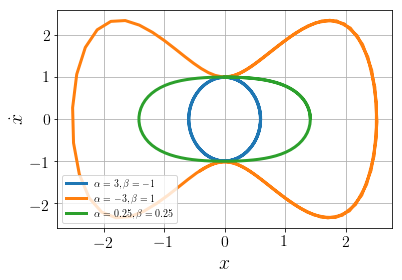
\includegraphics[scale=0.7]{1c.png}
\end{figure}

\textbf{Part (d)}
$$E= mv^2/2 + \alpha x^2/2 + \beta x^4/4$$
$$\therefore v = \sqrt{\frac{2}{m}(E- \alpha x^2/2 - \beta x^4/4)}$$

At the turning points, $x$ will satisfy,
\begin{flalign*}
\alpha x^2/2 + \beta x^4/4 &= E\\
\alpha x^2/2 + \beta x^4/4 - E &= 0\\
\end{flalign*}
\text{The (possibly real) roots of which are }
$$x_1 = \sqrt{\frac{\sqrt{\alpha ^2+4 e \beta }}{\beta }-\frac{\alpha }{\beta }} \text{ and } x_2= - \sqrt{\frac{\sqrt{\alpha ^2+4 e \beta }}{\beta }-\frac{\alpha }{\beta }}$$

We know that,

$$v = \derivative{x}{t} \ , \  \therefore T = 2\int_{x2}^{x_1} \frac{1}{v}dx = 2\int_{x2}^{x_1} \frac{1}{\sqrt{\frac{2}{m}(E- \alpha x^2/2 - \beta x^4/4)}}dx$$

Using Mathematica to evaluate the indefinite integral, we get,



$$v = -2 \eval{-\frac{i \sqrt{\frac{\beta  x^2}{\alpha -\sqrt{\alpha ^2+4 \beta  \text{E}}}+1} \sqrt{\frac{x^2 \left(\sqrt{\alpha ^2+4 \beta  \text{E}}-\alpha \right)}{\text{E}}+4} F\left(i \sinh ^{-1}\left(x \sqrt{\frac{\beta }{\alpha -\sqrt{\alpha ^2+4 \text{E} \beta }}}\right)|\frac{\alpha -\sqrt{\alpha ^2+4 \text{E} \beta }}{\alpha +\sqrt{\alpha ^2+4 \text{E} \beta }}\right)}{\sqrt{\frac{\beta }{\alpha -\sqrt{\alpha ^2+4 \beta  \text{E}}}} \sqrt{\frac{8 \text{E}-2 \beta  x^4-4 \alpha  x^2}{m}}}}_{x_2}^{x_1}$$

where $F(x)$ is the \textit{elliptic integral of the first kind} and
$$x_1 = \sqrt{\frac{\sqrt{\alpha ^2+4 e \beta }}{\beta }-\frac{\alpha }{\beta }} \text{ and } x_2= - \sqrt{\frac{\sqrt{\alpha ^2+4 e \beta }}{\beta }-\frac{\alpha }{\beta }}$$

\textbf{Part (e)} - \textit{code files attached}\\

\textbf{Part (f)}\\
Substituting $x = A \cos(\omega t + \phi)$ in $m\ddot{x} + \delta \dot{x} + \alpha x  = \gamma \cos(\omega t) $
\begin{flalign*}
	(-m\omega^2 + \alpha )\cos(\omega t + \phi) - \delta \omega \sin(\omega t + \phi) = \frac{\gamma}{A}\cos(\omega t)
\end{flalign*}	
Expanding the RHS and equating coefficients of $\cos(\omega t)$ and $\sin(\omega t)$, one gets
$$(-m\omega^2 + \alpha )\cos(\phi) - \delta \omega \sin(\phi) = \frac{\gamma}{A}$$
$$-(-m\omega^2 + \alpha )\sin(\phi) - \delta \omega \cos(\phi) = 0$$
Solving these, we get
$$A = \frac{\gamma}{\sqrt{\left(\alpha-m \omega ^2\right)^2+\delta^2 \omega ^2}} \text{ ; } \phi = \tan^{-1} \left(\frac{\delta \omega}{\alpha - m\omega^2}\right)$$

These are plotted below
\begin{figure}[h]
	\centering
	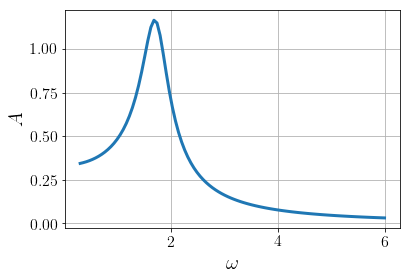
\includegraphics[scale=0.5]{A_om.png}
	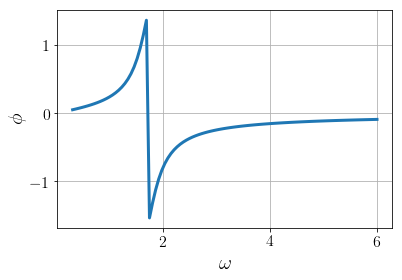
\includegraphics[scale=0.5]{p_om.png}
\end{figure}

\textbf{Part (g)}\\
The equation to be solved now is $$m \ddot{x}(t)-\gamma  \cos (t \omega )+\delta  x'(t)+\alpha  x(t)+\beta  x(t)^3 = 0$$
Again, Substituting $x = A \cos(\omega t + \phi)$
$$3 A^3 \beta  \cos (t \omega +\phi )+A^3 \beta  \cos (3 t \omega +3 \phi )-4 A m \omega ^2 \cos (t \omega +\phi )+4 \alpha  A \cos (t \omega +\phi )-4 A \delta  \omega  \sin (t \omega +\phi )-4 \gamma  \cos (t \omega ) = 0$$

Expanding this in terms of trigonometric functions of $n \omega t$ and equating the coeffiecients of $\cos (\omega t)$ and $\sin(\omega t)$ to zero,

$$\frac{3}{4} A^3 \beta  \cos (\phi )+\alpha  A \cos (\phi )-A \omega ^2 \cos (\phi )-\delta  \omega  \sin (\phi ) = \gamma$$

$$\frac{3}{4} A^3 \beta  \sin (\phi )-\alpha  A \sin (\phi )+A \omega ^2 \sin (\phi )-\delta  \omega  \cos (\phi ) = 0$$

Solving the above two for the amplitude $A$, we get,
$$\frac{9 A^6 \beta ^2}{16}+\frac{3}{2} \alpha  A^4 \beta -\frac{3}{2} A^4 \beta  \omega ^2+\alpha ^2 A^2-2 \alpha  A^2 \omega ^2+A^2 \omega ^4+\delta ^2 \omega ^2 = \gamma^2$$
This is the governing equation for $A$.
\\

\textbf{Part (h)} - \textit{code files attached}\\
\end{homeworkProblem}


\begin{homeworkProblem}
	\textit{Solved completely in the attached code files}
\end{homeworkProblem}

\begin{homeworkProblem}
	\textbf{Part (a)}\\
	Let $(R_1,v_1)$ and $(R_2,v_2)$ be the separation and velocity and the perigee and apogee respectively. write the energy and momentum conservation equations at the apogee and perigee,
	$$m v_1 R_1 = m v_2 R_2 \implies v_1 = \frac{R_2}{R_1} v_2 = \frac{1+e}{1-e}v_2$$
	$$\frac{m v_1^2}{2} - \frac{GMm}{R_1} = \frac{m v_2^2}{2} - \frac{GMm}{R_2}$$
	Substituting for $v_1$ in the energy conservation equation, along with $R_1$ and $R_2$,
	$$ GMm\frac{R_1 - R_2}{R_2 R_1} = \frac{m v_2^2}{2} \left[1 - \left(\frac{R_2}{R_1}\right)^2\right]$$
	$$ GM\frac{2R_1}{R_2 (R_1 + R_2)} = v_2^2$$
	
	But the energy $E$ is just given by,
	\begin{flalign*}
	E &= \frac{m v_2^2}{2} - \frac{GMm}{R_2}\\
	&=  -\frac{GMm}{R_2}\left(\frac{R_2}{R_1 + R_2}\right)\\
	&=  -\frac{GMm}{R_1 + R_2}\\
	E&=  -\frac{GMm}{2R}\
	\end{flalign*}

	
	\textbf{Part (b)}\\
	The qualitative mechanism to change the orbit can be described as follows :-
	\begin{itemize}
		\item When the satellite is at apogee, it is given an impulse which changes the orbit into an ellipse of perigee separation equal to the current apogee separation ie. $R(1+e)$, and apogee separation $2R$.
		
		\item Then when the satellite is at the new apogee separation, it is given an impulse such that its orbit is changed into a circle of radius $2R$.
	\end{itemize}
	
	\textbf{Part (c)}\\
	Let us calculate the momentum imparted in each of the stages described above:-
	
	\begin{itemize}
		\item Using the formula derived in the first part, the energy is the new orbit is just
		$$E = -\frac{GMm}{R(3+e)}$$
		The change in energy is purely change in kinetic energy. Hence the new velocity is,
		
		\begin{flalign*}
			v^2 &= v_i^2 + \frac{2}{m}\Delta E\\
			&= \frac{GM(1-e)}{R(1+e)} + \frac{2}{m} \left( \frac{GMm}{2R} - \frac{GMm}{R(3+e)}\right)\\
			&= \frac{GM(1-e)}{R(1+e)} + \frac{2}{m}  \frac{GMm}{R}\left(\frac{1}{2} - \frac{1}{(3+e)}\right)\\
			&= \frac{GM(1-e)}{R(1+e)} + \frac{2}{m}  \frac{GMm}{R}\left(\frac{1+e}{2(3+e)}\right)\\
			&= \frac{GM(1-e)}{R(1+e)} +  \frac{GM}{R}\left(\frac{1+e}{3+e}\right)\\
			&= \frac{4GM}{R(1+e)(3+e)}\\
			v &= \sqrt{\frac{4GM}{R(1+e)(3+e)}}
		\end{flalign*}
		The impulse imparted in this step is,
		$$I_1= m \sqrt{\frac{GM}{R(1+e)}}\left[ \sqrt{\frac{4}{(3+e)}}-\sqrt{1-e}\right]$$
		\item The energy in the final orbit will be,
		$$E = -\frac{GMm}{4R}$$ and the final velocity will be,
		$$v_f = \sqrt{\frac{GM}{2R}}$$
		The impulse in this step can be calculated in a similar fashion and it is
		$$I_2= m{\sqrt{\frac{GM}{R}}}\left[\displaystyle{\sqrt{\frac{1}{2}} -\sqrt{\frac{(1+e)}{(3+e)}}}\right]$$
	\end{itemize}

	Total Impulse imparted to the satellite , \\
	$$I_{total} = I_1 + I_2$$
	 $$I_{total} = \displaystyle{ m \sqrt{\frac{GM}{R}}\left[ \frac{1}{\sqrt{2}} - \sqrt{\frac{(1+e)}{(3+e)}} +\frac{2}{\sqrt{(3+e)(1+e)}} - \sqrt{\frac{(1-e)}{(1+e)}}\right]}$$

	\textbf{Part (d)}\\
	
	Initial Angular Momentum,
	$$L_i = m v_2 R_2$$
	$$L_i = m \sqrt{GMR(1 - e^2)}$$
	
	Final Angular Momentum,
	$$L_f = 2m v_f R$$
	$$L_f = m\sqrt{2GMR}$$
	
	Hence, change in angular momentum,
	$$\Delta L = L_f - L_i = m\sqrt{GMR} (\sqrt{2}-\sqrt{1-e^2})$$
\end{homeworkProblem}

\begin{homeworkProblem}
	\textit{Solved completely in the attached code files}
\end{homeworkProblem}
\end{document}
